\documentclass[12pt]{article}
% Full article preamble (duplicated, no common file)
\usepackage{fontspec}
\usepackage[a4paper,margin=2.5cm,includefoot]{geometry}
\usepackage{polyglossia}
\usepackage{amsmath}
\usepackage{amssymb}
\usepackage{xcolor}
\usepackage{fancyhdr}
\usepackage{graphicx}
\usepackage{listings}
\usepackage[most]{tcolorbox}
\usepackage{pifont}
\usepackage{enumitem}
\usepackage{titlesec}
\usepackage[bottom]{footmisc}
\usepackage{titling}
\usepackage{minted}
\usepackage{etoolbox}
\usepackage{array}
\usepackage{extsizes}

\newfontfamily\emoji{Segoe UI Emoji}

\pagestyle{fancy}

\setmainlanguage[numerals=western]{arabic}
\setotherlanguage{english}
\newfontfamily\arabicfont[Script=Arabic]{Amiri}
\newfontfamily\arabicfonttt[Script=Arabic]{Courier New}

\lstset{
  language=[Sharp]C,
  numbers=left,
  stepnumber=1,
  numbersep=8pt,
  frame=single,
  basicstyle=\ttfamily\small,
  keywordstyle=\color{blue},
  stringstyle=\color{red},
  commentstyle=\color{green!50!black}
}

\newif\ifdetailed
\ifdefined\setdetailed
  \setdetailed
\fi

\newif\ifwithsols
\ifdefined\setwithsols
  \setwithsols
\fi

% unified tcolorboxes for articles
\tcbset{colback=white, colframe=black, fonttitle=\bfseries, boxrule=0.8pt}
\newtcolorbox{boxDef}[1][]{colback=blue!5!white,colframe=blue!75!black,
  title={{\emoji📘} تعريف\ifx\\#1\\\else ~#1\fi :}}
\newtcolorbox{boxExercise}[1][]{colback=cyan!5!white,colframe=cyan!70!black,
  title={{\emoji🧩} تمرين\ifx\\#1\\\else ~#1\fi :}}
\newtcolorbox{boxExample}[1][]{colback=yellow!5!white,colframe=orange!90!black,
  title={{\emoji📝} مثال\ifx\\#1\\\else ~#1\fi :}}
\newtcolorbox{boxNote}[1][]{colback=gray!10!white,colframe=black,
  title={{\emoji✨} ملاحظة\ifx\\#1\\\else ~#1\fi :}}
\newtcolorbox{boxAttention}[1][]{colback=magenta!10!white,colframe=magenta!80!black,
  title={{\emoji🔔} تنبيه\ifx\\#1\\\else ~#1\fi :}}
\newtcolorbox{boxWarning}[1][]{colback=red!5!white,colframe=red!75!black,
  title={{\emoji⚡} ملاحظة هامة\ifx\\#1\\\else ~#1\fi :}}
\newtcolorbox{boxSolution}[1][]{colback=green!5!white,colframe=green!60!black,
  title={{\emoji✅} حل\ifx\\#1\\\else ~#1\fi :}}
\newtcolorbox{boxSymbol}[1][]{colback=purple!5!white,colframe=purple!70!black,
  title={{\emoji🔣} رمز\ifx\\#1\\\else ~#1\fi :}}

\tcbset{simplecode/.style={ colback=gray!5, colframe=black!50, boxrule=0.4pt, arc=2pt, left=4pt,right=4pt,top=4pt,bottom=4pt}}
\newenvironment{boxCode}{\begin{tcolorbox}[simplecode]}{\end{tcolorbox}}

\newcolumntype{C}[1]{>{\centering\arraybackslash}p{#1}}

% redefine spaces after titles
\makeatletter
\renewcommand{\@maketitle}{%
  \begin{center}
    {\huge \bfseries \@title \par}%
    \vskip 0.2em % space between title and author
    {\large \@author \par}%
    % \vskip 0.2em % space between author and date
    % {\normalsize \@date \par}%
  \end{center}
}
\makeatother

\fancyhf{} % clear default
\fancypagestyle{plain}{
  \fancyhf{}
  \fancyhead[L]{مدرسة التسامح الشاملة}
  % \fancyhead[L]{
\includegraphics[height=1cm]{../../../images/logoTasamoh.png}}
  \fancyhead[R]{الأستاذ محمود اغبارية}
  \fancyfoot[C]{\thepage}
}

\fancyhead[L]{مدرسة التسامح الشاملة}
\fancyhead[R]{الأستاذ محمود اغبارية}
\fancyfoot[C]{\thepage}
% \date{\today}

\setcounter{tocdepth}{3} % only section subsection and subsubsection in TOC


% ----------------------


% \begin{document}

% \maketitle

% % \clearpage  % start TOC on a new page
% % \renewcommand{\contentsname}{جدول المحتويات}
% % \tableofcontents
% % \clearpage

% \part*{part 1} % the * prevents numbering
% \section*{مقدمة}
% \subsection*{مثال رياضي}
% \subsubsection*{مثال فرعي}
% \paragraph*{ paragraph 1}
% \subparagraph*{sub paragraph 1}

% \ifdetailed
% \begin{english}
% \begin{minted}{csharp}
% // C# Example
% \end{minted}
% \end{english}
% \fi

% OLD WAY
% \ifdetailed
% \begin{english}
% \begin{lstlisting}
% // C# Example
% \end{lstlisting}
% \end{english}
% \fi

% % 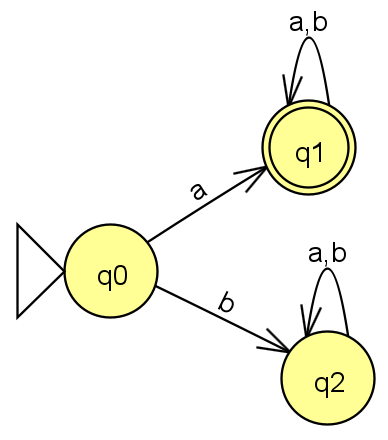
\includegraphics[width=0.2\textwidth]{../../../images/DFAs/ex1_q1.png}



% \vspace{3cm}
% \begin{flushleft}
% أرجو لكم وقتًا ممتعًا.

% الأستاذ محمود اغبارية.
% \end{flushleft}


% \end{document}


\begin{document}

\title{أسئلة للمراجعة قبل الامتحان}

\maketitle
\thispagestyle{fancy}

\begin{enumerate}[itemsep=2em]

\item
	اكتب مقطع برنامج يستقبل ثلاثة أعداد صحيحة، على البرنامج أن يحسب ويطبع معدل هذه العلامات.\\
     \begin{boxExample}
     إذا كانت الأعداد الثلاثة هي 7, 15, 6 فالمعدل هو 9.333.
     \end{boxExample}

\ifwithsols
\begin{boxSolution}
\begin{english}
\begin{minted}{csharp}
Console.Write("Enter three integers: ");
int a = int.Parse(Console.ReadLine());
int b = int.Parse(Console.ReadLine());
int c = int.Parse(Console.ReadLine());
double avg = (a + b + c) / 3.0;
Console.WriteLine($"Average = {avg}");
\end{minted}
\end{english}
\end{boxSolution}
\fi

\item
	اكتب مقطع برنامج يستقبل طول وعرض مستطيل ما، على البرنامج أن يحسب ويطبع مساحة ومحيط المستطيل. \\
    \begin{boxExample}
    إذا كان الطول يساوي 6 والعرض يساوي 4 فالمساحة هي $6 \cdot 4 = 24$، والمحيط هو $ (6 + 4) \cdot 2 = 20$.
    \end{boxExample}

\ifwithsols
\begin{boxSolution}
\begin{english}
\begin{minted}{csharp}
Console.Write("Enter rectangle length: ");
int length = int.Parse(Console.ReadLine());
Console.Write("Enter rectangle width: ");
int width = int.Parse(Console.ReadLine());
int area = length * width;
int perimeter = 2 * (length + width);
Console.WriteLine($"Area = {area}");
Console.WriteLine($"Perimeter = {perimeter}");
\end{minted}
\end{english}
\end{boxSolution}
\clearpage
\fi

\item
	حدّد صح أو خطأ مع الشرح لكل أمر من الأوامر التالية:
\begin{english}
    \begin{enumerate}
	\item \texttt{int x = 7.0;}     \underline{\hspace{7cm}}
	\item \texttt{double y = 2.0, c = 4;}   \underline{\hspace{7cm}}
	\item \texttt{string s1 = hi friends;}  \underline{\hspace{7cm}}
	\item \texttt{int x1 = 11;}  \underline{\hspace{7cm}}
    \item \texttt{double num = x1 – 4;}   \underline{\hspace{7cm}}
	\item \texttt{double h = 3.17;}  \underline{\hspace{7cm}}
    \item \texttt{int f = h;}  \underline{\hspace{7cm}}
	\item \texttt{char ch1 = 'L';}  \underline{\hspace{7cm}}
	\item \texttt{char ch2 = '?2s';}   \underline{\hspace{7cm}}

\end{enumerate}
\end{english}

\ifwithsols
\begin{boxSolution}
\begin{itemize}
  \item \texttt{int x = 7.0;} خطأ — \texttt{7.0} عدد عشري لا يمكن إسناده إلى \texttt{int} دون تحويل صريح.
  \item \texttt{double y = 2.0, c = 4;} صحيح — كلاهما من النوع \texttt{double} (\texttt{4} يُحوَّل إلى \texttt{4.0}).
  \item \texttt{string s1 = hi friends;} خطأ — يجب إحاطة النص بعلامتي اقتباس: \texttt{"hi friends"}.
  \item \texttt{int x1 = 11;} صحيح.
  \item \texttt{double num = x1 – 4;} صحيح إذا كان الرمز ناقص عادي \texttt{-} (أحيانًا يُكتب خطأً كشرطة طويلة). النتيجة \texttt{double}.
  \item \texttt{double h = 3.17;} صحيح.
  \item \texttt{int f = h;} خطأ — لا يمكن إسناد \texttt{double} إلى \texttt{int} دون تحويل صريح.
  \item \texttt{char ch1 = 'L';} صحيح.
  \item \texttt{char ch2 = '?2s';} خطأ — الحرف الواحد فقط داخل \texttt{'}\,\texttt{'}. يجب استخدام \texttt{"?2s"} كسلسلة.
\end{itemize}
\end{boxSolution}
\fi

\clearpage
\item
	اكتب مقطع برنامج يستقبل كمُدخل عددين صحيحين، على البرنامج أن يحسب ويطبع حاصل جمع وحاصل طرح وحاصل ضرب وحاصل قسمة وحاصل باقي قسمة العددين، كل نتيجة بسطر مختلف كما في المثال أدناه.
\begin{boxExample}
    إذا كان العددان هما 2, 9 البرنامج يطبع بالشكل التالي:
    \begin{align*}
        &9 + 2 = 11 \\
        &9 - 2 = 7 \\
        &9 * 2 = 18 \\
        &9 / 2 = 4 \\
        &9 \% 2 = 1
    \end{align*}
\end{boxExample}

\ifwithsols
\begin{boxSolution}
\begin{english}
\begin{minted}{csharp}
Console.Write("Enter first integer: ");
int a = int.Parse(Console.ReadLine());
Console.Write("Enter second integer: ");
int b = int.Parse(Console.ReadLine());
Console.WriteLine($"{a} + {b} = {a + b}");
Console.WriteLine($"{a} - {b} = {a - b}");
Console.WriteLine($"{a} * {b} = {a * b}");
Console.WriteLine($"{a} / {b} = {a / b}");
Console.WriteLine($"{a} % {b} = {a % b}");
\end{minted}
\end{english}
\end{boxSolution}
\clearpage
\fi

\item
	معطى البرنامج التالي:
\begin{english}
\begin{minted}{csharp}
public class Program
{
    Public static void Main()
    {
        Console.WriteLine("Enter num: ");
        double x = double.Parse(Console.ReadLine());

        Console.WriteLine("Enter num: ");
        double y = double.Parse(Console.ReadLine());

        double result = Math.Pow(x, 2) + Math.Pow(y, 3);
        Console.WriteLine(result);
    }
}
\end{minted}
\end{english}
\begin{enumerate}
    \item ماذا سيطبع البرنامج إذا أدخلنا إليه القيم \(x = 3\) و \(y = 2\)?
    \item ما هي وظيفة البرنامج أعلاه؟
    \item أعطِ مثالًا لقيم لـ $x$ و $y$ تجعل البرنامج يطبع: 5
\end{enumerate}

\ifwithsols
\begin{boxSolution}
\begin{itemize}
    \item البرنامج سيطبع 17.0
  \item وظيفة البرنامج: قراءة قيمتين \texttt{x}, \texttt{y} وحساب \(x^2 + y^2\) ثم طباعته.
  \item مثال لنتيجة 5: \(x = 2\), \(y = 1\) أو العكس.
\end{itemize}
\end{boxSolution}
\fi

\clearpage
\item
    في مطعم الطويل ثمن ساندويتش فلافل 15 شاقل وثمن ساندويتش شاورما 40 شاقل. \\
    اكتب مقطع برنامج يستقبل عدد ساندويتشات الفلافل وعدد ساندويتشات الشاورما التي باعها المطعم في أحد الأيام. \\
    على البرنامج أن يحسب ويطبع المدخول الكلي الذي جمعه المطعم في ذلك اليوم. \\
    \begin{boxExample}
        المطعم باع في ذلك اليوم 35 ساندويتش فلافل و 46 ساندويتش شاورما، مدخول المطعم: \\
        $$35 \cdot 15 + 46 \cdot 40 = 2365$$
    \end{boxExample}

\ifwithsols
\begin{boxSolution}
\begin{english}
\begin{minted}{csharp}
Console.Write("Falafel count: ");
int falafel = int.Parse(Console.ReadLine());
Console.Write("Shawarma count: ");
int shawarma = int.Parse(Console.ReadLine());
int income = falafel * 15 + shawarma * 40;
Console.WriteLine($"Total income = {income} NIS");
\end{minted}
\end{english}
\end{boxSolution}
\fi

    \item
	في محل لبيع الأجهزة الكهربائية يُدفع مبلغ الشراء بالطريقة التالية: \\
     نصف المبلغ نقدي والنصف الآخر يتم تقسيمه على خمسة أقساط. \\
      اكتب مقطع برنامج يستقبل الثمن الكلي للأجهزة الكهربائية التي اشتراها زبون ما، على البرنامج أن يحسب ويطبع المبلغ المدفوع نقدا وقيمة القسط الواحد.  \\
    \begin{boxExample}
        اذا كان الثمن الكلي هو 10000 شاقل فقيمة المبلغ النقدي هي: $\frac{10000}{2}=5000$ شاقل وقيمة القسط الواحد هي $\frac{5000}{5}=1000$ شاقل.
    \end{boxExample}

\ifwithsols
\begin{boxSolution}
\begin{english}
\begin{minted}{csharp}
Console.Write("Total price: ");
double total = double.Parse(Console.ReadLine());
double cash = total / 2.0;
double installment = cash / 5.0;
Console.WriteLine($"Cash = {cash}");
Console.WriteLine($"Each installment = {installment}");
\end{minted}
\end{english}
\end{boxSolution}
\clearpage
\fi

    \item
	اكتب مقطع برنامج يستقبل علامة الفصل الأول وعلامة الفصل الثاني وعلامة الفصل الثالث بموضوع علم الحاسوب، على البرنامج أن يحسب ويطبع معدل العلامات بالطريقة التالية:
     \%30 من علامة الفصل الأول، \%25 من علامة الفصل الثاني و \%45 من علامة الفصل الثالث. \\
     \begin{boxExample}
        إذا كانت علامة الفصل الأول 82 وعلامة الفصل الثاني 77 وعلامة الفصل الثالث 92, فالمعدل يكون: $0.3 \cdot 82 + 0.25 \cdot 77 + 0.45 \cdot 92 = 85.25$.
     \end{boxExample}

\ifwithsols
\begin{boxSolution}
\begin{english}
\begin{minted}{csharp}
Console.Write("First term grade: ");
double g1 = double.Parse(Console.ReadLine());
Console.Write("Second term grade: ");
double g2 = double.Parse(Console.ReadLine());
Console.Write("Third term grade: ");
double g3 = double.Parse(Console.ReadLine());
double avg = 0.30 * g1 + 0.25 * g2 + 0.45 * g3;
Console.WriteLine($"Weighted average = {avg}");
\end{minted}
\end{english}
\end{boxSolution}
\fi

     \item
	يمكن حساب مساحة مثلث أضلاعه a, b, c حسب القانون التالي:
    $$S_\Delta = \sqrt{p (p-a) (p-b) (p-c)}$$
    بحيث أنّ: $p=\frac{a+b+c}{2}$ \\
اكتب مقطع برنامج يستقبل كمدخل ثلاثة أضلاع مثلث ما، على البرنامج أن يطبع مساحته حسب القانون أعلاه.

\ifwithsols
\begin{boxSolution}
\begin{english}
\begin{minted}{csharp}
Console.Write("a: ");
double a = double.Parse(Console.ReadLine());
Console.Write("b: ");
double b = double.Parse(Console.ReadLine());
Console.Write("c: ");
double c = double.Parse(Console.ReadLine());
double p = (a + b + c) / 2.0;
double area = Math.Sqrt(p * (p - a) * (p - b) * (p - c));
Console.WriteLine($"Area = {area}");
\end{minted}
\end{english}
\end{boxSolution}
\clearpage
\fi

\item
	اكتب مقطع برنامج يستقبل عددًا رباعي المنزلة، على البرنامج أن يطبع حاصل جمع أول خانة مع آخر خانة. \\
    \begin{boxExample}
        بالنسبة للعدد 6321 يطبع: $6 + 1 = 7$.
    \end{boxExample}

\ifwithsols
\begin{boxSolution}
\begin{english}
\begin{minted}{csharp}
Console.Write("Enter four-digit number: ");
int n = int.Parse(Console.ReadLine());
int first = n / 1000;
int last = n % 10;
Console.WriteLine($"{first} + {last} = {first + last}");
\end{minted}
\end{english}
\end{boxSolution}
\fi

    \item
	اكتب مقطع برنامج يستقبل عددين صحيحين وموجبين ثنائيا المنزلة، على البرنامج أن يطبع حاصل ضرب خانة الآحاد من العدد الأول بخانة العشرات من العدد الثاني. \\
    \begin{boxExample}
        إذا كان العدد الأول 24، والعدد الثاني 87، فعلى البرنامج أن يطبع 32، لأنّ $4 \cdot 8 = 32$.
    \end{boxExample}

\ifwithsols
\begin{boxSolution}
\begin{english}
\begin{minted}{csharp}
Console.Write("Enter two two-digit positives: ");
int n1 = int.Parse(Console.ReadLine());
int n2 = int.Parse(Console.ReadLine());
int onesFirst = n1 % 10;
int tensSecond = (n2 / 10) % 10;
Console.WriteLine(onesFirst * tensSecond);
\end{minted}
\end{english}
\end{boxSolution}
\clearpage
\fi

\item
	اكتب مقطع برنامج يستقبل عددين ثلاثيي المنزلة، على البرنامج أن يطبع حاصل جمع تكعيب خانة العشرات بالعدد الاول مع تكعيب خانة العشرات بالعدد الثاني. \\
    \begin{boxExample}
    بالنسبة للعددين 176 و 420 البرنامج يطبع: $7^3 + 2^3 = 351$.
    \end{boxExample}

\ifwithsols
\begin{boxSolution}
\begin{english}
\begin{minted}{csharp}
Console.Write("Enter two three-digit numbers: ");
int m1 = int.Parse(Console.ReadLine());
int m2 = int.Parse(Console.ReadLine());
int tens1 = (m1 / 10) % 10;
int tens2 = (m2 / 10) % 10;
int sum = Math.Pow(tens1, 3) + Math.Pow(tens2, 3);
Console.WriteLine(sum);
\end{minted}
\end{english}
\end{boxSolution}
\fi

    \item
	اكتب مقطع برنامج يستقبل عددًا رباعي المنزلة، على البرنامج أن يقسّم العدد الى عددين ثنائيي المنزلة: عدد مؤلف من خانتي الآحاد والعشرات وعدد مؤلف من خانتي المئات والآلاف. \\
    البرنامج يطبع حاصل طرح العدد الصغير من العدد الكبير. \\
    \begin{boxExample}
        بالنسبة للعدد 6781 العددان هما 81 و 67 والبرنامج يطبع: $81 - 67 = 14$.
    \end{boxExample}

\ifwithsols
\begin{boxSolution}
\begin{english}
\begin{minted}{csharp}
Console.Write("Enter four-digit number: ");
int k = int.Parse(Console.ReadLine());
int low = k % 100;       // ones+tens
int high = k / 100;      // hundreds+thousands
int big = Math.Max(low, high);
int small = Math.Min(low, high);
Console.WriteLine(big - small);
\end{minted}
\end{english}
\end{boxSolution}
\fi

\clearpage
    \item
	في مصنع لإنتاج حبات الشوكولاتة يعبئون كل 30 حبة بعلبة. \\
    اكتب مقطع برنامج يستقبل عدد حبات الشوكولاتة التي أنتجها المصنع في أحد الايام، على البرنامج أن يطبع عدد العُلب التي ملأها المصنع ذلك اليوم، وأيضًا يطبع عدد حبّات الشوكولاتة التي بقيت ولم تكفِ لملء علبة إضافية. \\
    \begin{boxExample}
        بالنسبة لـ 3070 حبة، فإنّ المصنع ملأ 102 عُلب كاملة، وبقيت 10 حبّات لم تُملأ لأنّها لم تكفِ لعلبة إضافية.
    \end{boxExample}

\ifwithsols
\begin{boxSolution}
\begin{english}
\begin{minted}{csharp}
Console.Write("Enter number of chocolates: ");
int total = int.Parse(Console.ReadLine());
int boxes = total / 30;
int rem = total % 30;
Console.WriteLine($"Boxes filled = {boxes}");
Console.WriteLine($"Leftover = {rem}");
\end{minted}
\end{english}
\end{boxSolution}
\clearpage
\fi

\item
عدد مميز هو عدد ثنائي المنزلة يقسم على مجموع خاناته. \\
مثلًا، العدد 12 هو عدد مميّز لأنّ مجموع خاناته هو $1+2=3$، و 12 يقسم على 3. \\
اكتب برنامجًا يستقبل عددًا صحيحًا، على البرنامج أن يطبع:
\begin{itemize}
    \item \textenglish{ERROR} إذا لم يكن العدد من  منزلتين (أي إذا كان من منزلة واحدة، أو من ثلاث منازل فأكثر)
    \item \textenglish{Special} إذا كان العدد من منزلتين، وكان عددًا مميّزًا
    \item \textenglish{Not Special} إذا كان العدد من منزلتين، لكنه غير مميّز
\end{itemize}
\begin{boxExample}[1]
    إذا كان العدد 24، فالبرنامج يطبع: \\
    \textenglish{Special}
    (لأنّ $24/6=4$)
\end{boxExample}
\begin{boxExample}[2]
    إذا كان العدد 5  أو  345 فالبرنامج يطبع: \\
    \textenglish{ERROR}
\end{boxExample}
\begin{boxExample}[3]
    إذا كان العدد 13 فالبرنامج يطبع: \\
    \textenglish{Not special}
\end{boxExample}

\ifwithsols
\begin{boxSolution}
\begin{english}
\begin{minted}{csharp}
int num = int.Parse(Console.ReadLine());
if (num < 10 || num > 99)
{
    Console.WriteLine("ERROR");
}
else
{
    int sum = num / 10 + num % 10;
    if (num % sum == 0)
    {
        Console.WriteLine("Special");
    }
    else
    {
        Console.WriteLine("Not Special");
    }
}
\end{minted}
\end{english}
\end{boxSolution}
\fi

\end{enumerate}
\end{document}
